\header{
    \section{Le bon roi Dagobert} \label{le-bon-roi-dagobert}
    %
    
    \insertComment{Version paillarde d'une chanson populaire publiée en 1861.}{Le roi Dagobert a régné de 629 à 638 aux côtés de Saint Eloi, un orfèvre probablement référencé dans la chanson "Les 3 orfèvres"}
}

\enluminure{4}{\href{https://www.youtube.com/watch?v=jvAhXi5oMAE}{L}}{e bon} roi Dagobert
\\Baisait à tort et à travers.
\\Le grand Saint-Eloi
\\Lui dit: "Oh mon roi,
\\Votre Majesté va se fatiguer."
\\"Cochon", lui dit le roi
\\"Tu voudrais bien foutre pour moi".
\\\\Le bon roi Dagobert
\\Enfilait les femmes à l'envers.
\\Le grand Saint-Eloi
\\Lui dit: "Oh mon roi,
\\Vous êtes entré du mauvais côté".
\\"Crétin", lui dit le roi
\\"Tu sais bien que l'envers vaut l'endroit".
\\\\C'est le roi Dagobert,
\\Qui bandait toujours comme un cerf
\\Le grand Saint-Eloi
\\Lui dit: "Oh mon roi,
\\On voit votre gland c'n'est pas élégant".
\\Le roi dit aussitôt:
\\"Oh ! je vais y accrocher mon chapeau".
\\\\Le bon roi Dagobert
\\Avait toujours la queue à l'air
\\Le grand Saint-Eloi
\\Lui dit: "Oh mon roi,
\\Au mois de décembre faut rentrer son membre".
\\Le roi lui dit, très fier:
\\"Rien ne vaut le vit au grand air".
\breakpage
Le bon roi Dagobert
\\Etait demeuré très primaire
\\Au grand Saint-Eloi
\\Qui lui demanda :
\\"Dites-moi au moins c'que font un et un?"
\\Il gueula comme un boeuf:
\\"Un et un, ça fait soixante-neuf".
\\\\Le bon roi Dagobert
\\Se faisait sucer au dessert
\\La reine fort choquée
\\Lui dit: "c'est assez,
\\Devant tout le palais, c'est vraiment très laid".
\\Le roi lui dit: "Souveraine,
\\On ne doit pas parler la bouche pleine".
\\\\Le bon roi Dagobert
\\En mourant fit cette prière:
\\"Mon cher Saint-Eloi,
\\Je voudrais ma foi
\\Que l'on mît à part mon grand braquemart".
\\"Il servira d'ailleurs
\\De sceptre à tous mes successeurs".
\begin{center}
   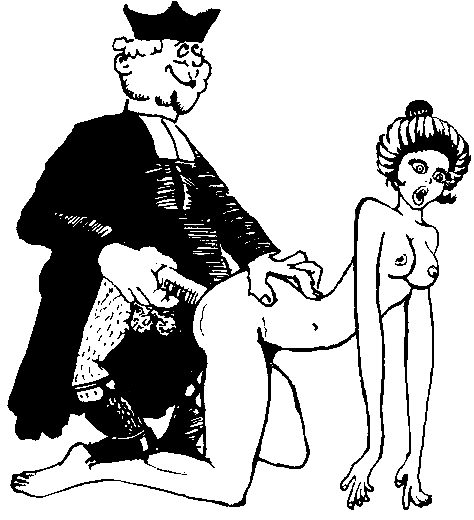
\includegraphics[width=0.6\textwidth]{images/dagobert.png}
 \end{center}
\breakpage